\documentclass[12pt]{beamer}
\usepackage{../Estilos/BeamerMAF}
\usetheme{Dresden}
\usecolortheme{seahorse}
%\useoutertheme{default}
\setbeamercovered{invisible}
% or whatever (possibly just delete it)
\setbeamertemplate{section in toc}[sections numbered]
\setbeamertemplate{subsection in toc}[subsections numbered]
\setbeamertemplate{subsection in toc}{\leavevmode\leftskip=3.2em\rlap{\hskip-2em\inserttocsectionnumber.\inserttocsubsectionnumber}\inserttocsubsection\par}
\setbeamercolor{section in toc}{fg=blue}
\setbeamercolor{subsection in toc}{fg=blue}
\setbeamercolor{frametitle}{fg=blue}
\setbeamertemplate{caption}[numbered]

\setbeamertemplate{footline}
\beamertemplatenavigationsymbolsempty
\setbeamertemplate{headline}{}

\makeatletter
\setbeamercolor{section in foot}{bg=gray!30, fg=black!90!orange}
\setbeamercolor{subsection in foot}{bg=blue!30!yellow, fg=red}
\setbeamertemplate{footline}
{
  \leavevmode%
  \hbox{%
  \begin{beamercolorbox}[wd=.333333\paperwidth,ht=2.25ex,dp=1ex,center]{section in foot}%
    \usebeamerfont{section in foot} \insertsection
  \end{beamercolorbox}}%
  \begin{beamercolorbox}[wd=.333333\paperwidth,ht=2.25ex,dp=1ex,center]{subsection in foot}%
    \usebeamerfont{subsection in foot}  \insertsubsection
  \end{beamercolorbox}%
  \begin{beamercolorbox}[wd=.333333\paperwidth,ht=2.25ex,dp=1ex,right]{date in head/foot}%
    \usebeamerfont{date in head/foot} \insertshortdate{} \hspace*{2em}
    \insertframenumber{} / \inserttotalframenumber \hspace*{2ex} 
  \end{beamercolorbox}}%
  \vskip0pt%
\makeatother 

\makeatletter
\patchcmd{\beamer@sectionintoc}{\vskip1.5em}{\vskip0.8em}{}{}
\makeatother


\setbeamercolor{section in foot}{bg=ballblue, fg=black}
\setbeamercolor{subsection in foot}{bg=bronze, fg=black}
\setbeamercolor{date in foot}{bg=goldenrod, fg=white}

\makeatletter
\setbeamertemplate{footline}
{
\leavevmode%
\hbox{%
\begin{beamercolorbox}[wd=.333333\paperwidth,ht=2.25ex,dp=1ex,center]{section in foot}%
  \usebeamerfont{section in foot} \insertsection
\end{beamercolorbox}%
\begin{beamercolorbox}[wd=.333333\paperwidth,ht=2.25ex,dp=1ex,center]{subsection in foot}%
  \usebeamerfont{subsection in foot}  \insertsubsection
\end{beamercolorbox}%
\begin{beamercolorbox}[wd=.333333\paperwidth,ht=2.25ex,dp=1ex,right]{date in head/foot}%
  \usebeamerfont{date in head/foot} \insertshortdate{} \hspace*{1.5em}
  \insertframenumber{} / \inserttotalframenumber \hspace*{2ex} 
\end{beamercolorbox}}%
\vskip0pt%
}
\makeatother
\usefonttheme{serif}
\resetcounteronoverlays{saveenumi}

\date{19 de abril de 2022}

\title{\large{Completes en eigenfunciones}}
\subtitle{Tema 3 - Bases completas y ortogonales}
\author{M. en C. Gustavo Contreras Mayén}


\begin{document}
\maketitle
\fontsize{14}{14}\selectfont
\spanishdecimal{.}

\section*{Contenido}
\frame[allowframebreaks]{\tableofcontents[currentsection, hideallsubsections]}

%Ref. Arfken (2006) 10.4
\section{3a. propiedad Op. autoadjuntos}
\frame{\tableofcontents[currentsection, hideothersubsections]}
\subsection{Completes de las eigenfunciones}

\begin{frame}
\frametitle{La tercera propiedad por revisar}
La tercera propiedad importante de un operador autoadjunto (Hermitiano) consiste en que \emph{las eigenfunciones forman un conjunto completo}.
\end{frame}
\begin{frame}
\frametitle{La tercera propiedad por revisar}  
Esta completes significa que cualquier función bien portada (al menos en partes pero continua) $F (x)$ se puede aproximar por una serie:
\pause
\begin{align}
F (x) = \nsum_{n=0}^{\infty} a_{n} \, \phi_{n} (x) 
\label{eq:ecuacion_10_62}
\end{align}
con cualquier grado de precisión.
\end{frame}
\begin{frame}
\frametitle{Precisión en el concepto}
Con mayor formalismo, el conjunto $\phi_{n} (x)$ se dice que es \textbf{completo}, si en el límite el error medio cuadrado se anula:
\pause
\begin{align}
\lim_{m \to \infty} \scaleint{6ex}_{\bs a}^{b} \bigg[ F (x) - \nsum_{n=0}^{m} a_{n} \, \phi_{n} (x) \bigg]^{2} \, \sigma (x) \dd{x} = 0
\label{eq:ecuacion_10_63}
\end{align}
\end{frame}
\begin{frame}
\frametitle{Precisión en el concepto}
Técnicamente, esta es una integral de Lebesgue.
\\
\bigskip
\pause
No necesariamente el error es nulo en $[a,b]$, pero sólo la integral del error al cuadrado debe ser cero.
\end{frame}
\begin{frame}
\frametitle{Relevancia de la convergencia}
La convergencia en la media (ec. \ref{eq:ecuacion_10_63}) debe compararse con la convergencia uniforme.
\\
\bigskip
\pause
La convergencia uniforme implica la convergencia en la media, pero de manera inversa no se garantiza, la convergencia en la media es menos restrictiva.
\end{frame}
\begin{frame}
\frametitle{Funciones válidas}
En la ecuación (\ref{eq:ecuacion_10_63}) no es válida para funciones continuas en piezas, ya que hay un número finito de discontinuidades.
\\
\bigskip
\pause
Un ejemplo relevante es \emph{el fenómeno de Gibbs} de las series discontinuas de Fourier, que también ocurre para otras series de funciones propias.
\end{frame}
\begin{frame}
\frametitle{$f (x) = \mbox{sign } (x) \in [-\pi, \pi]$}
\begin{figure}
  \centering
  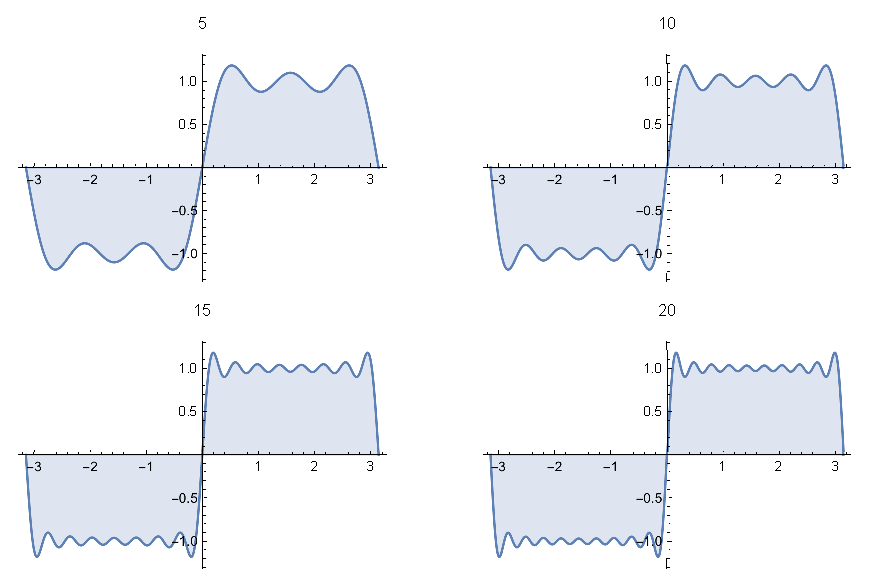
\includegraphics[scale=0.7]{Imagenes/Gibbs_Fourier.eps}
\end{figure}
\end{frame}
\begin{frame}
\frametitle{Calculando los coeficientes}
En la ecuación (\ref{eq:ecuacion_10_62}) la expansión de los coeficientes $a_{m}$ se determinar mediante:
\pause
\begin{align}
a_{m} = \scaleint{5ex}_{\bs a}^{b} F(x) \, \phi_{m}^{*} (x) \, \sigma (x) \dd{x}
\label{eq:ecuacion_10_64}
\end{align}
\pause
Que se obtiene al multiplicar la ecuación (\ref{eq:ecuacion_10_62}) por $\phi_{m}^{*} (x) \, \sigma (x)$ y luego se integra.
\end{frame}
\begin{frame}
\frametitle{Usando la ortogonalidad}
De la ortogonalidad de las eigenfunciones $\phi_{n}(x)$, solo el $m$-ésimo término sobrevive, por lo que la ortogonalidad es importante.
\\
\bigskip
\pause
La ecuación (\ref{eq:ecuacion_10_64}) puede compararse con el producto interno de vectores. \pause En ocasiones los coeficientes $a_{m}$ son llamados \textbf{coeficientes generalizados de Fourier}.
\end{frame}
\begin{frame}
\frametitle{Calculando los coeficientes}
Para una función conocida $F (x)$, la ecuación (\ref{eq:ecuacion_10_64}) proporciona los $a_{m}$ como una \textbf{integral definida} que siempre se puede evaluar, ya sea numéricamente si es que no es de manera analítica.
\end{frame}
\begin{frame}
\frametitle{Equivalencia lineal}
En términos del álgebra lineal, tenemos un espacio lineal, un espacio de funciones.
\\
\bigskip
\pause
Las funciones linealmente independientes, ortonormales $\phi_{n} (x)$ forman una base de ese espacio (infinito-dimensional).
\end{frame}
\begin{frame}
\frametitle{Espacio de Hilbert}
La ecuación (\ref{eq:ecuacion_10_62}) es un punto que nos dice que las funciones $\phi_{n} (x)$ cubre ese espacio lineal.
\\
\bigskip
\pause
Con un producto punto definido por la ec. (\ref{eq:ecuacion_10_64}), el espacio lineal que tenemos, se convierte en un \textbf{espacio de Hilbert}.
\end{frame}
\begin{frame}
\frametitle{Uso conveniente de $\sigma (x)$}
Por simplicidad, dejando la función de peso $\sigma (x) = 1$, la cerradura en forma de un operador para un conjunto discreto de eigenfunciones $\ket{\phi_{i}}$ es:
\pause
\begin{align*}
\setlength{\fboxsep}{3\fboxsep}\boxed{
\nsum_{i} \ket{\varphi_{i}} \bra{\varphi_{i}} =  1}
\end{align*}
\end{frame}
\begin{frame}
\frametitle{Usando un ket}
Multiplicando la relación de cerradura por $\ket{F}$ obtenemos la expansión de la eigenfunción:
\pause
\begin{align*}
\setlength{\fboxsep}{3\fboxsep}\boxed{
\ket{F} = \nsum_{i} \ket{\phi_{i}} \braket{\phi_{i}}{F}}
\end{align*}
con el coeficiente generalizado de Fourier $a_{i} = \braket{\phi_{i}}{F}$.
\end{frame}
\begin{frame}
\frametitle{Representación coordenada}
De manera equivalente en una representación coordenada:
\pause
\begin{align*}
\setlength{\fboxsep}{3\fboxsep}\boxed{
\nsum_{i} \phi_{i}^{*} (y) \, \phi_{i} (x) = \delta (x - y)}
\end{align*}
\end{frame}
\begin{frame}
\frametitle{Representación coordenada}
Implica que:
\begin{eqnarray*}
\begin{aligned}
F(x) &= \scaleint{5ex} \, F(y) \, \delta (x - y) \, \dd{y} = \\[0.5em] \pause
&= \nsum_{i} \phi_{i} (x) \, \scaleint{5ex} \, \phi_{i}^{*} (y) \, F(y) \dd{y}
\end{aligned}
\end{eqnarray*}
\end{frame}
\begin{frame}
\frametitle{Una apuesta}
Sin pruebas, afirmamos que el espectro de un operador lineal $A$ que mapea un espacio de Hilbert $\mathcal{H}$ en sí mismo \pause puede dividirse en un espectro discreto (o puntual) con eigenvectores de longitud finita.
\end{frame}
\begin{frame}
\frametitle{Espectro continuo}
Un espectro continuo para que la ecuación de eigenvalores $A \, v = \lambda \, v$ con $v$ en $\mathcal{H}$ no tiene una inversa acotada única $(A - \lambda)^{-1}$ en un dominio denso de $\mathcal{H}$.
\\
\bigskip
\pause
Y un espectro residual donde $(A - \lambda)^{-1}$ está no acotado en un dominio no denso en $\mathcal{H}$.
\end{frame}

\subsection{Desigualdad de Bessel}

\begin{frame}
\frametitle{Definición}
Si el conjunto de funciones $\phi_{n} (x)$ \emph{no forma un conjunto completo}, \pause posiblemente sea por que no se han incluido el número infinito de elementos del conjunto completo, esto nos conduce a la \emph{desigualdad de Bessel}.
\end{frame}
\begin{frame}
\frametitle{Caso finito}
Consideremos primero un caso finito. Sea $\vb{A}$ un vector de $n$ componentes:
\pause
\begin{align}
\vb{A} = \vu{e}_{1} \, a_{1} + \vu{e}_{2} \, a_{2} + \ldots + \vu{e}_{n} \, a_{n} 
\label{eq:ecuacion_10_66}
\end{align}
en donde $\vu{e}_{i}$ es un vector unitario y $a_{i}$ es la correspondiente componente (proyección) de $\vb{A}$.
\end{frame}
\begin{frame}
\frametitle{Componentes del vector $\vb{A}$}
Esto es:
\pause
\begin{align}
a_{i} = \vb{A} \cdot \vu{e}_{i}
\label{eq:ecuacion_10_67}
\end{align}
\pause
Entonces:
\pause
\begin{align}
\left( \vb{A} - \nsum_{i} \vu{e}_{i} \, a_{i} \right)^{2} \geq 0
\label{eq:ecuacion_10_68}
\end{align}
\end{frame}
\begin{frame}
\frametitle{Interpretando la desigualdad}
Si sumamos todos los $n$ componentes, evidentemente la suma se iguala a $\vb{A}$ por la ecuación (\ref{eq:ecuacion_10_66}) y la igualdad es consistente.
\\
\bigskip
\pause
Pero cuando la suma no incluye a todos los $n$ componentes, resulta la desigualdad.
\end{frame}
\begin{frame}
\frametitle{Usando la ortogonalidad}
Expandiendo la ecuación (\ref{eq:ecuacion_10_68}) y eligiendo los vectores unitarios para que satisfagan la relación de ortogonalidad:
\pause
\begin{align}
\vu{e}_{i} \cdot \vu{e}_{j} = \delta_{ij}
\label{eq:ecuacion_10_69}
\end{align}
\end{frame}
\begin{frame}
\frametitle{La desigualdad de Bessel}
Tenemos que:
\pause
\begin{align}
\vb{A}^{2} \geq \nsum_{i} a_{i}^{2}
\label{eq:ecuacion_10_70}
\end{align}
Que es \underline{la desigualdad de Bessel}.
\end{frame}
\begin{frame}
\frametitle{Caso continuo}
Para funciones reales debemos de considerar la integral:
\pause
\begin{align}
\scaleint{7ex}_{\bs a}^{b} \left[ f (x) - \nsum_{i} a_{i} \, \phi_{i} (x) \right]^{2} \, \sigma (x) \dd{x} \geq 0
\label{eq:ecuacion_10_71}
\end{align}
que es el análogo continuo de la ecuación (\ref{eq:ecuacion_10_68}), haciendo $n \to \infty$ y reemplazando la suma por la integración.
\end{frame}
\begin{frame}
\frametitle{Consideraciones de la integral}
Nuevamente, con el factor de peso $\sigma (x) > 0 $, el integrando es no negativo.
\\
\bigskip
\pause
La integral se anula por la ecuación (\ref{eq:ecuacion_10_62}) si tenemos un conjunto completo. \pause De otra forma, es positiva.
\end{frame}
\begin{frame}
\frametitle{Detallando la expresión}
Desarrollando el término al cuadrado obtenemos:
\pause
\begin{equation}
\begin{aligned}
\scaleint{5ex}_{\bs a}^{b} \big[ f (x) \big]^{2} \, \sigma (x) \dd{x} &- 2 \nsum_{i} a_{i} \, \scaleint{5ex}_{\bs a}^{b} f (x) \, \phi (x) \, \sigma (x) \dd{x} + \\[0.5em]
&+ \nsum_{i} a_{i}^{2} \geq 0
\end{aligned}
\label{eq:ecuacion_10_72}
\end{equation}
\end{frame}
\begin{frame}
\frametitle{Ocupando un resultado}
Usando la ecuación (\ref{eq:ecuacion_10_64}), tenemos:
\pause
\begin{equation}
\scaleint{5ex}_{\bs a}^{b} \big[ f (x) \big]^{2} \, \sigma (x) \dd{x} \geq \nsum_{i} a_{i}^{2}
\label{eq:ecuacion_10_73}
\end{equation}
\end{frame}
\begin{frame}
\frametitle{El caso con los coeficientes}
De aquí que la suma de los cuadrados de la expansión de los coeficientes $a_{i}$ es menor o igual que la integral ponderada de $[f (x)]^{2}$, \pause la igualdad se mantiene si y sólo si, \pause la expansión es exacta, \pause esto ocurre si el conjunto de soluciones $\phi_{n} (x)$ es un conjunto completo.
\end{frame}
\begin{frame}
\frametitle{La relación de Parseval}
Cuando se considera que las eigenfunciones que forman conjuntos completos (como los polinomios de Legendre), la ec. (\ref{eq:ecuacion_10_73}) con el signo igual que se mantiene se llamará \textbf{relación de Parseval}.
\\
\bigskip
\pause
La desigualdad de Bessel tiene distintos usos, incluida la prueba de convergencia para las series de Fourier.
\end{frame}

\subsection{Desigualdad de Schwarz}

\begin{frame}
\frametitle{Uso de la desigualdad}
La desigualdad de Schwarz de uso frecuente es similar a la desigualdad de Bessel.
\\
\bigskip
\pause
Consideremos la ecuación cuadrática con la incógnita $x$:
\begin{align}
\nsum_{i=1}^{n} (a_{i} \, x + b_{i})^{2} = \nsum_{i=1}^{n} a_{i}^{2} \left( x + \dfrac{b_{i}}{a_{i}} \right)^{2} = 0
\label{eq:ecuacion_10_74}
\end{align}
con $a_{i}$, $b_{i}$ reales.
\end{frame}
\begin{frame}
\frametitle{Casos en el cociente}
\setbeamercolor{item projected}{bg=blue!70!black,fg=yellow}
\setbeamertemplate{enumerate items}[circle]
\begin{enumerate}[<+->]
\item Si $b_{i}/a_{i}$ es la constante $c$, independiente del índice $i$, la solución es $x= - c$.
\item Si $b_{i}/a_{i}$ no es constante en $i$, todos los términos no se anulan simultáneamente para un $x$ real, por lo que la solución debe de ser compleja.
\end{enumerate}
\end{frame}
\begin{frame}
\frametitle{Expandiendo los términos}
Expandiendo, tenemos que:
\pause
\begin{align}
x^{2} \, \nsum_{i}^{n} a_{i}^{2} + 2 \, x \, \nsum_{i}^{n} a_{i} \, b_{i} + \nsum_{i}^{n} b_{i}^{2} = 0
\label{eq:ecuacion_10_75}
\end{align}
\end{frame}
\begin{frame}
\frametitle{En el caso complejo}
Como $x$ es complejo (o = $-b_{i}/a_{i}$), la fórmula cuadrática para $x$ conduce a:
\pause
\begin{align}
\left( \nsum_{i=1}^{n} a_{i} \, b_{i} \right)^{2} \leq \left( \nsum_{i=1}^{n} a_{i}^{2} \right) \, \left( \nsum_{i=1}^{n} b_{i}^{2} \right)
\label{eq:ecuacion_10_76}
\end{align}
la igualdad se mantiene cuando $b_{i}/a_{i}$ es una constante independiente de $i$.
\end{frame}
\begin{frame}
\frametitle{Caso discreto}
Nuevamente, en términos de vectores, tenemos:
\pause
\begin{align}
( \vb{a} \cdot \vb{b} )^{2} =  a^{2} \, b^{2} \, \cos^{2} \theta \leq a^{2} \, b^{2}
\label{eq:ecuacion_10_77}
\end{align}
donde $\theta$ es el ángulo entre $\vb{a}$ y $\vb{b}$.
\end{frame}
\begin{frame}
\frametitle{La desigualdad de Schwarz compleja}
La desigualdad de Schwarz para funciones complejas tiene la expresión:
\pause
\begin{align}
\begin{aligned}[b]
&\abs{ \scaleint{5ex}_{\bs a}^{b} f^{*} (x) \, g (x) \dd{x} }^{2} \leq \\[0.5em]
&\leq \scaleint{5ex}_{\bs a}^{b} f^{*} (x) \, f (x) \dd{x} \scaleint{5ex}_{\bs a}^{b} g^{*} (x) \, g (x) \dd{x}
\end{aligned}
\label{eq:ecuacion_10_78}
\end{align}
\end{frame}
\begin{frame}
\frametitle{Interpretando la desigualdad}
La desigualdad se mantiene si y sólo si:
\begin{align*}
g (x) = \alpha \, f (x)
\end{align*}
siendo $\alpha$ una constante.
\end{frame}
\begin{frame}
\frametitle{Interpretando la desigualdad}
Para probar esta forma de la función de la desigualdad de Schwarz, consideremos la función compleja:
\pause
\begin{align*}
\psi (x) = f(x) + \lambda \, g (x)
\end{align*}
con $\lambda$ una constante compleja, donde las funciones $f (x)$ y $g (x)$ son cualesquiera dos funciones de cuadrado integrable (para las cuales, las integrales del lado derecho existen).
\end{frame}
\begin{frame}
\frametitle{Manejando la expresión}
Multiplicando por el conjugado complejo y luego integrando, tenemos:
\pause
\begin{align}
\begin{aligned}
\scaleint{5ex}_{\bs a}^{b} \psi^{*} \, \psi \dd{x} &\equiv \scaleint{5ex}_{\bs a}^{b} f^{*} \, f \dd{x} + \lambda \, \int_{a}^{b} f^{*} \, g \dd{x} + \\[0.5em]
&+ \lambda^{*} \, \scaleint{5ex}_{\bs a}^{b} g^{*} \, f \dd{x} + \\
&+ \lambda \, \lambda^{*} \, \scaleint{5ex}_{\bs a}^{b} g^{*} \, g \, \dd{x}  \geq 0
\end{aligned}
\label{eq:ecuacion_10_79}
\end{align}
\end{frame}
\begin{frame}
\frametitle{Interpretando la desigualdad}
\setbeamercolor{item projected}{bg=blue!70!black,fg=yellow}
\setbeamertemplate{enumerate items}[circle]
\begin{enumerate}[<+->]
\item El $\geq 0$ aparece ya que $\psi^{*} \, \psi$ es no negativo.
\item El signo igual $(=)$ se mantiene sólo si $\psi (x)$ es idéntico a cero.
\end{enumerate}
\end{frame}
\begin{frame}
\frametitle{Minimizando la expresión}
Nótese que $\lambda$ y $\lambda^{*}$ son linealmente independientes, \pause diferenciamos con respecto a uno de ellos, \pause e igualamos la derivada a cero para minimizar $\displaystyle \int_{a}^{b} \psi^{*} \, \psi \dd{x}$:
\pause
\begin{align*}
\pdv{\lambda^{*}} \scaleint{5ex}_{\bs a}^{b} \psi^{*} \, \psi \dd{x} = \scaleint{5ex}_{\bs a}^{b} g^{*} \, f \dd{x}  + \lambda \scaleint{5ex}_{\bs a}^{b} g^{*} g \dd{x} = 0
\end{align*}
\end{frame}
\begin{frame}
\frametitle{Resultado de la minimización}
Que nos lleva a:
\pause
\begin{align}
\lambda = - \, \dfrac{\displaystyle \scaleint{5ex}_{\bs a}^{b} g^{*} \, f \dd{x}}{\displaystyle \scaleint{5ex}_{\bs a}^{b} g^{*} \, g \dd{x}}
\label{eq:ecuacion_10_80a}
\end{align}
\end{frame}
\begin{frame}
\frametitle{Usando el conjugado complejo}
Tomando el conjugado complejo:
\pause
\begin{align}
\lambda^{*} = - \dfrac{\displaystyle \scaleint{5ex}_{\bs a}^{b} f^{*} \, g \dd{x}}{\displaystyle \scaleint{5ex}_{\bs a}^{b} g^{*} \, g \dd{x}}
\label{eq:ecuacion_80b}
\end{align}
\end{frame}
\begin{frame}
\frametitle{Sustituyendo los resultados}
Sustituyendo esos valores de $\lambda$ y $\lambda^{*}$ en la ecuación (\ref{eq:ecuacion_10_79}), \pause obtenemos la ecuación (\ref{eq:ecuacion_10_78}), \underline{la desigualdad de Schwarz}.
\end{frame}
\begin{frame}
\frametitle{Ejemplo de la mecánica cuántica}
En mecánica cuántica las funciones $f (x)$ y $g (x)$ podrían representar un estado o una configuración de un sistema físico, es decir, una combinación lineal de funciones de onda.
\end{frame}
\begin{frame}
\frametitle{Utilidad de la desigualdad de Schwarz}
Entonces la desigualdad e Schwarz garantiza que el producto punto $\displaystyle \int_{a}^{b} f^{*} (x) \, g(x) \, \dd{x}$ existe.
\\
\bigskip
\pause
En algunos textos, la desigualdad de Schwarz es un paso para llegar al principio de incertidumbre de Heisenberg.
\end{frame}
\begin{frame}
\frametitle{Mejorando la escritura}
La notación de las funciones de las ecuaciones (\ref{eq:ecuacion_10_78}) y (\ref{eq:ecuacion_10_79}) es a veces incómoda; \pause en mecánica cuántica es común utilizar la notación de Dirac.
\end{frame}
\begin{frame}
\frametitle{Simplificando la escritura}
Con esta notación, se simplifica tanto el rango de integración $(a, b)$, como la función de peso $\sigma (x) \geq 0$. 
\\
\bigskip
\pause
La desigualdad de Schwarz ahora se representa:
\pause
\begin{align}
\abs{\braket{f}{g}}^{2} \leq \braket{f}{f} \, \braket{g}{g}
\label{eq:ecuacion_10_78a}
\end{align}
\end{frame}
\begin{frame}
\frametitle{Caso con una eigenfunción}
Si $g (x)$ es una eigenfunción normalizada, $\phi_{i} (x)$, la ecuación (\ref{eq:ecuacion_10_78}) nos lleva a (donde $\sigma (x) = 1$):
\pause
\begin{align}
a_{i}^{*} \, a_{i} \leq \scaleint{5ex}_{\bs a}^{b} f^{*} (x) \, f (x) \dd{x} 
\label{eq:ecuacion_10_81}
\end{align}
Que es un resultado que se sigue de la ecuación (\ref{eq:ecuacion_10_73}).
\end{frame}

% %Ref. Arfken (1981) pág. 514

\section{Representación con la delta de Dirac}
\frame{\tableofcontents[currentsection, hideothersubsections]}
\subsection{Eigenfunciones y la delta de Dirac}

\begin{frame}
\frametitle{Las eigenfunciones y la $\delta$ de Dirac}
El conjunto ortonormal de eigenfunciones $\phi_{n} (x)$ proporciona otra representación interesante de la función delta de Dirac.
\end{frame}
\begin{frame}
\frametitle{Una suma de utilidad}
Consideremos la suma:
\pause
\begin{align}
K (x, t) = K (t, x) = \nsum_{n=0}^{\infty} \phi_{n} (x) \, \phi_{n} (t)
\label{eq:ecuacion_09_80}
\end{align}
Por conveniencia, se supone que $\phi_{n} (x)$ se ha definido para incluir $[\sigma (x)]^{1/2}$ si $\sigma (x) \neq 1$.
\end{frame}
\begin{frame}
\frametitle{Consideración importante}
Esta serie en la ec. (\ref{eq:ecuacion_09_80}) de hecho no es convergente uniformemente, \pause pero puede utilizarse como parte de un integrando en donde la integración subsecuente la convierta en convergente.
\end{frame}
\begin{frame}
\frametitle{Preparando una integral}
Supongamos ahora que se forma la integral:
\pause
\begin{align*}
\scaleint{6ex} F (t) \, K (x, t) \dd{t}
\end{align*}
en donde se considera que $F (t)$ se puede desarrollar en serie de eigenfunciones $\phi_{p} (t)$.
\end{frame}
\begin{frame}
\frametitle{Estudiando la integral}
Se tiene que:
\pause
\begin{eqnarray}
\begin{aligned}[b]
\scaleint{6ex} &F (t) \, K (x, t) \dd{t} = \\[0.5em] \pause
&= \scaleint{6ex} \nsum_{p=0}^{\infty} a_{p} \, \phi_{p} (t) \, \nsum_{n=0}^{\infty} \phi_{n} (x) \, \phi_{n} (t) \dd{t} = \\[0.5em] \pause
&= \nsum_{p=0}^{\infty} a_{p} \, \phi_{p} (x) = \pause F (x)
\end{aligned}
\label{eq:ecuacion_09_81}
\end{eqnarray}
en que los productos opuestos $\phi_{p} \, \phi_{n} \, (n \neq p)$ desaparecen por ortogonalidad.
\end{frame}
\begin{frame}
\frametitle{Usando la definición de la $\delta (x)$}
Al tomar en cuenta la definición de la función delta de Dirac, el resultado de la ec. (\ref{eq:ecuacion_09_81}) significa que:
\pause
\begin{align}
K (x, t) = \delta (x - t) = \nsum_{n=0}^{\infty} \phi_{n} (x) \, \phi_{n} (t)
\label{eq:ecuacion_09_82}
\end{align}
\end{frame}
\begin{frame}
\frametitle{Resultado fácil de demostrar}
Es fácil demostrar que:
\pause
\begin{align}
\scaleint{6ex} K (x, t) \dd{t} = 1
\label{eq:ecuacion_09_83}
\end{align}
permitiendo que $F (t) = \phi_{0}$, una constante.
La confirmación del comportamiento en $x = t$ se encuentra al utilizar la desigualdad de Bessel.
\end{frame}
\begin{frame}
\frametitle{La función con el mismo argumento}
Se tiene que:
\pause
\begin{align}
K (t, t) = \nsum_{n=0}^{\infty} \big[ \phi_{n} (t) \big]^{2}
\label{eq:ecuacion_09_84}
\end{align}
\end{frame}
\begin{frame}
\frametitle{Sustituyendo una expresión}
Usando la ec. (\ref{eq:ecuacion_10_73}), se obtiene:
\pause
\begin{align}
\scaleint{6ex} \big[ K (t, t) \big]^{2} \dd{t} = \nsum_{n=0}^{\infty} a_{n}^{2} = \nsum_{n=0}^{\infty} 1 = \infty
\label{eq:ecuacion_09_85}
\end{align}
En consecuencia, $K(x, t)$ diverge en $x = t$, tal como era de esperarse.
\end{frame}

% %Ref. Arfken 10.5 (2006)

\section{Función de Green}
\frame{\tableofcontents[currentsection, hideothersubsections]}
\subsection{Expansión en eigenfunciones}

\begin{frame}
\frametitle{La función de Green}
Una serie algo similar a la representada por $K (x, t)$ - que es a la vez $\delta (x - t)$ - \pause resulta cuando se desarrolla la función de Green en eigenfunciones de la ecuación homogénea correspondiente.
\end{frame}
\begin{frame}
\frametitle{La ecuación de Helmholtz}
En la ecuación de Helmholtz no homogénea se tiene que:
\pause
\begin{align}
\setlength{\fboxsep}{3\fboxsep}\boxed{
\laplacian \psi (\vb{r}) + k^{2} \, \psi (\vb{r}) = - \rho (\vb{r})
\label{eq:ecuacion_10_82}}
\end{align}
\end{frame}
\begin{frame}
\frametitle{La ec. de Helmholtz homogénea}
La ecuación de Helmholtz homogénea se satisface con sus eigenfunciones ortonormales $\varphi_{n}$:
\pause
\begin{align}
\laplacian \varphi_{n} (\vb{r}) + k_{n}^{2} \, \varphi_{n} (\vb{r}) = 0
\label{eq:ecuacion_10_83}
\end{align} 
\end{frame}
\begin{frame}
\frametitle{La función de Green}
La función de Green $G (\vb{r}_{1}, \vb{r}_{2})$ satisface la ecuación de la fuente en el punto:
\pause
\begin{align}
\setlength{\fboxsep}{3\fboxsep}\boxed{
\laplacian G (\vb{r}_{1}, \vb{r}_{2}) + k^{2} \, G (\vb{r}_{1}, \vb{r}_{2}) = - \delta (\vb{r}_{1}, \vb{r}_{2})}
\label{eq:ecuacion_10_84}
\end{align}
con las condiciones de frontera impuestas en las soluciones de la ecuación homogénea.
\end{frame}
\begin{frame}
\frametitle{Consideraciones de la función de Green}
Dado que $G$ es real, \pause se desarrolla la función de Green en la forma de serie de funciones propias de la ecuación homogénea, ec. (\ref{eq:ecuacion_10_83}), es decir:
\pause
\begin{align}
G (\vb{r}_{1}, \vb{r}_{2}) = \nsum_{n=0}^{\infty} a_{n} (\vb{r}_{2}) \, \varphi_{n} (\vb{r}_{1})
\label{eq:ecuacion_10_85}
\end{align}
\end{frame}
\begin{frame}
\frametitle{Sustituyendo el resultado}
Que al sustituir en la ec. (\ref{eq:ecuacion_10_84}), se obtiene:
\pause
\begin{align}
\begin{aligned}[b]
- \nsum_{n=0}^{\infty} &a_{n} (\vb{r}_{2}) k_{n}^{2} \varphi_{n} (\vb{r}_{1}) + k^{2} \nsum_{n=0}^{\infty} a_{n} (\vb{r}_{2}) \varphi_{n} (\vb{r}_{1}) = \\[0.5em]
&- \nsum_{n=0}^{\infty} \varphi_{n} (\vb{r}_{1}) \, \varphi_{n} (\vb{r}_{2})
\end{aligned}
\label{eq:ecuacion_10_86}
\end{align}
Aquí, la $\delta (\vb{r}_{1} - \vb{r}_{2})$ se ha sustituido por su desarrollo de eigenfunción.
\end{frame}
\begin{frame}
\frametitle{Usando la ortogonalidad}
Cuando se utiliza la ortogonalidad de $\varphi_{n} (\vb{r}_{1})$ para aislar $a_{n}$, nos lleva a:
\pause
\begin{align*}
&\nsum_{m=0}^{\infty} a_{m} (\vb{r}_{2}) \, \big( k_{n}^{2} - k_{m}^{2} \big) \, \scaleint{6ex} \varphi_{n} (\vb{r}_{1}) \, \varphi_{m} (\vb{r}_{1}) \dd[3]{r_{1}} = \\[0.5em]
&- \nsum_{n=0}^{\infty} \varphi_{m} (\vb{r}_{2})  \, \scaleint{6ex} \varphi_{n} (\vb{r}_{1}) \, \varphi_{m} (\vb{r}_{1}) \dd[3]{r_{1}}    
\end{align*} 
\end{frame}
\begin{frame}
\frametitle{Expresión alterna}
De manera equivalente:
\pause
\begin{align*}
a_{n} (\vb{r}_{2}) \, \big( k^{2} - k_{n}^{2} \big) = - \varphi_{n} (\vb{r}_{2})
\end{align*}
\end{frame}
\begin{frame}
\frametitle{Sustityuendo de nuevo}
Que al sustituir en la ec. (\ref{eq:ecuacion_10_85}), la función de Green se transforma en:
\pause
\begin{align}
\setlength{\fboxsep}{3\fboxsep}\boxed{
G (\vb{r}_{1}, \vb{r}_{2}) = \nsum_{n=0}^{\infty} \dfrac{\varphi_{n} (\vb{r}_{1}) \, \varphi_{n} (\vb{r}_{2})}{k_{n}^{2} - k^{2}}}
\label{eq:ecuacion_10_87}
\end{align}
que es un desarrollo bilineal, simétrico con respecto a $\vb{r}_{1}$ y $\vb{r}_{2}$ como era de esperarse.
\end{frame}
\begin{frame}
\frametitle{La solución esperada}
Finalmente, $\psi (\vb{r}_{1})$, la solución deseada para la ecuación no homogénea está dada por:
\pause
\begin{align}
\setlength{\fboxsep}{3\fboxsep}\boxed{
\psi (\vb{r}_{1}) = \scaleint{6ex} G (\vb{r}_{1}, \vb{r}_{2}) \, \rho (\vb{r}_{2}) \dd{\tau_{2}}}
\label{eq:ecuacion_10_88}
\end{align}
\end{frame}
\begin{frame}
\frametitle{Generalizando lo encontrado}
Si se generaliza la ecuación diferencial no homogénea a:
\pause
\begin{align}
\mathcal{L} \psi + \lambda \, \psi = - \rho
\label{eq:ecuacion_10_89}
\end{align}
en donde $\mathcal{L}$ es el operador Hermitiano.
\end{frame}
\begin{frame}
\frametitle{Resultado}
Se tiene que:
\pause
\begin{align}
G (\vb{r}_{1}, \vb{r}_{2}) = \nsum_{n=0}^{\infty} \dfrac{\varphi_{n} (\vb{r}_{1}) \, \varphi_{n} (\vb{r}_{2})}{\lambda_{n} - \lambda}
\label{eq:ecuacion_10_90}
\end{align}
\end{frame}
\begin{frame}
\frametitle{Eigenvalores y eigenfunciones}
En donde $\lambda_{n}$ es el n-ésimo eigenvalor de $\varphi_{n}$, \pause la eigenfunción normal correspondiente a la ED homogénea:
\pause
\begin{align}
\mathcal{L} \, \psi + \lambda \, \psi = 0
\label{eq:ecuacion_10_91}
\end{align}
\end{frame}
\begin{frame}
\frametitle{Propiedad de simetría}
La expansión en eigenfunciones de la función de Green en la ec. (\ref{eq:ecuacion_10_90}) hace explícita la propiedad de simetría:
\pause
\begin{align*}
G (\vb{r}_{1}, \vb{r}_{2}) = G (\vb{r}_{2}, \vb{r}_{1})
\end{align*}
y es útil cuando se compara con soluciones obtenidas por otros medios.
\end{frame}

\section{Ejercicios y Examen}
\frame{\tableofcontents[currentsection, hideothersubsections]}
\subsection{Ejercicios a cuenta}

\begin{frame}
\frametitle{Ejercicio 9 para completar el Tema 3}
%Ref. Arfken 10.4.4
\textbf{Ejercicio 9. } En lugar de la expansión de una función $F(x)$ dada por:
\begin{align*}
F(x) = \nsum_{n=0}^{\infty} a_{n} \, \varphi_{n} (x)
\end{align*}
con los coeficientes:
\begin{align*}
a_{n} = \scaleint{5ex}_{\bs a}^{b} F(x) \, \varphi_{n} (x) \, \omega (x) \dd{x}
\end{align*}
\end{frame}
\begin{frame}
\frametitle{Ejercicio 9 para completar el Tema 3}
Considera la aproximación por una serie \textbf{finita}:
\begin{align*}
F(x) \approx \nsum_{n=0}^{m} c_{n} \, \varphi_{n} (x)
\end{align*}
\end{frame}
\begin{frame}
\frametitle{Ejercicio 9 para completar el Tema 3}
Demuestra que el cuadrado del error medio:
\begin{align*}
\scaleint{5ex}_{\bs a}^{b} \bigg[ F(x) - \nsum_{n=0}^{m} c_{n} \, \varphi_{n} (x) \bigg]^{2} \, \omega (x) \dd{x}
\end{align*}
se minimiza cuando $c_{n} = a_{n}$.
\end{frame}
\begin{frame}
\frametitle{Nota para el ejercicio}
\emph{Nota: } Los valores de los coeficientes son independientes del número de términos en la serie finita. Esta independencia es una consecuencia de la ortogonalidad y no sería válida para un ajuste por mínimos cuadrados utilizando potencias de $x$.
\end{frame}
\begin{frame}
\frametitle{Ejercicio 10 para el Tema 3}
%Ref. Arfken 10.4.7
\textbf{Ejercicio 10. } Recupera la desigualdad de Schwarz de la siguiente identidad:
\begin{align*}
&\bigg[ \scaleint{5ex}_{\bs a}^{b} f(x) \, g(x) \dd{x} \bigg
]^{2} {=} \scaleint{5ex}_{\bs a}^{b} \big[ f(x) \big
]^{2} \dd{x} \, \scaleint{5ex}_{\bs a}^{b} \big[ g(x) \big
]^{2} \dd{x} + \\[0.5em]
&- \dfrac{1}{2} \, \scaleint{5ex}_{\bs a}^{b} \, \scaleint{5ex}_{\bs a}^{b} \bigg[ f(x) \, g(y) - f(y) \, g(x) \bigg
]^{2} \dd{x} \dd{y}
\end{align*}
\end{frame}
\begin{frame}
\frametitle{Observación para el ejercicio}
\emph{Nota:} Cuida el signo de la expresión, recuerda que al cortar el renglón, se deja el signo $+$, en el siguiente renglón se tiene el signo $-$, por lo que el segundo término está restando el producto del primer término.
\end{frame}

\subsection{Enunciado para el Examen}

\begin{frame}
\frametitle{Enunciado Examen Intermedio}
La representación de la función delta de Dirac:
\begin{align*}
\delta (x - t) = \nsum_{n=0}^{\infty} \varphi_{n} (x) \, \varphi_{n} (t)
\end{align*}
frecuentemente se denomina \emph{relación de cierre.}
\end{frame}
\begin{frame}
\frametitle{Enunciado Examen Intermedio}
Para un conjunto ortonormal de funciones $\varphi_{n}$, demuestra que el cierre implica la completes, es decir, que la ecuación:
\begin{align*}
F (x) = \nsum_{n=0}^{\infty} a_{n} \, \varphi_{n} (x)
\end{align*}
se deriva de la expresión que define la $\delta (x - t)$.
\end{frame}
\begin{frame}
\frametitle{Fecha de entrega}
Los ejercicios pendientes y el enunciado del Tema 3 del examen intermedio, se deberán de entregar \textbf{el martes 26 de abril a las 6 pm} por Moodle.
\end{frame}
\end{document}